\documentclass{article}
\usepackage[utf8]{inputenc}
\usepackage{tikz}
\usepackage{circuitikz}
\usepackage{enumitem}
\usepackage{amsmath}
\usetikzlibrary{calc}
\usetikzlibrary{positioning,shapes.gates.logic.US}

\title{EC-2014-2}
\author{dilip}
\date{January 2021}

\begin{document}

\maketitle

\section{Question}

\begin{figure}[h]
    \centering
    \scalebox{0.65}{
    \begin{tikzpicture}[
        GateCfg/.style={
            logic gate inputs={normal,normal,normal},
            draw,
            scale=1.5
        }
    ]
    
    % D flip flop 1
    \draw (0,0)coordinate (A)--++(0:3.5)coordinate (B)--++(90:4.5)coordinate (C)--++(180:3.5)coordinate (D)--cycle;
    \draw ($(A)!0.8!(D)$)node[right]{\Large D}--++(180:1.5)node[]{};
    \draw ($(A)!0.5!(C)$)node[]{\Large D Latch};
    \draw ($(B)!0.8!(C)$)node[left]{\Large Q}--++(0:4)node[]{};
    \draw ($(B)!0.2!(C)$)node[left]{\Large $\overline{\mbox{Q}}$}--++(0:0.5)node[]{};
    \draw ($(A)!0.53!(D)$)node[]{}--++(-30:0.3)node[]{}--++(-150:0.3)node[]{};
    \draw ($(A)!0.5!(D)$)node[]{}--++(180:1.5)node[]{};
    
    % D flip flop 2
    \draw (7.5,0)coordinate (A)--++(0:3.5)coordinate (B)--++(90:4.5)coordinate (C)--++(180:3.5)coordinate (D)--cycle;
    \draw ($(A)!0.8!(D)$)node[right]{\Large Q};
    \draw ($(A)!0.5!(C)$)node[]{\Large Q Latch};
    \draw ($(B)!0.8!(C)$)node[left]{\Large Q}--++(0:1.5)node[]{};
    \draw ($(B)!0.2!(C)$)node[left]{\Large $\overline{\mbox{Q}}$}--++(0:1.5)node[]{};
    \draw ($(A)!0.53!(D)$)node[]{}--++(-30:0.3)node[]{}--++(-150:0.3)node[]{};
    \draw ($(A)!0.5!(D)$)node[]{}--++(180:1.5)node[]{};
    
    % CLK
    \draw (-2.5,-1)node[below]{\Large CLK}node[]{}--++(0:1)node[]{}--++(90:3.25)node[]{};
    
    \draw (2,-1)node[not gate US,GateCfg](NOT){};
    \draw (-1.5,-1)node[]{}--(NOT.input)node[]{};
    \draw (NOT.output)node[]{}--++(0:3.35)node[]{}--++(90:3.27)node[]{};
    
\end{tikzpicture} }
    \caption{Question Diagram}
    \label{fig:my_label}
\end{figure}

Current option is

\begin{enumerate}[label=(\alph*)]
    \item JK flip-flop
    \item SR flip-flop
    \item D flip-flop
    \item Master-slave arrangement
\end{enumerate}

\section{Answer} 
 The correct option is d)Master-slave arrangement
 \subsection{Master-Slave D flip flop}
  The basic D-type flip flop can be improved further by adding a second SR flip flop to its output that is activated on the complementary clock signal to produce a "Master-Slave D-type flip flop".On the leading edge of the clock signal( LOW-to-HIGH)the first stage, the "master" latches the input condition at D,while the output stage is deactivated.
  \paragraph{}
  On the trailing edge of the clock signal (HIGH-to-LOW), the second"slave" stage is now activated, latching on to the output from the first master circuit. Then the output stage appears to be triggered on the negative edge of the clock pulse." Master-Slave D-type flip flop" can be constructed by the cascading together of two latches with opposite clock phases as shown.
\begin{figure}[h]
\centering
\scalebox{0.7}{
  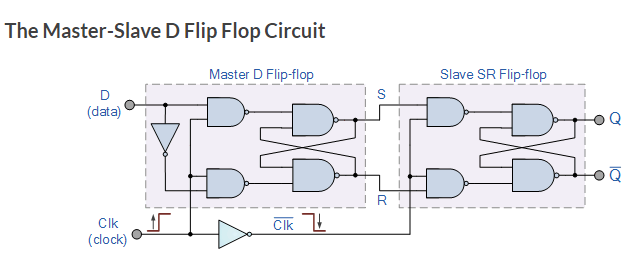
\includegraphics[]{circuit.png} }
\end{figure}
  \paragraph{}
  We can see from above that on the leading edge of the clock pulse the master flip-flop will be loading data from the data D input, therefore the master is "ON". With the trailing edge of the clock pulse, the slave flip-flop is loading data,i.e.the slave is "ON".Then there will always be one flip-flop"ON" and the other "OFF" but never both the master and slave "ON" at the same time.Therefore, the output Q acquires the value of D,only when one complete pulse,ie,0-1- is applied to clock input.
\end{document}
